\section{Introduction}

This chapter provides a detailed though non-exhaustive description of
the theory and techniques used in this thesis. First is an overview of
Algorithmic Skeletons, GPGPU programming, and the combination of the
two in SkelCL. Second is a description of the machine learning
techniques used in this thesis, followed by the tools and
methodologies used in the evaluation.


\section{Parallel Programming with Algorithmic Skeletons}

Introduced by \citeauthor{Cole1989} in \citeyear{Cole1989},
Algorithmic Skeletons simplify the task of parallel programming by
abstracting common patterns of communication, providing parallel
implementations of higher order functions~\cite{Cole1989}. The
interfaces to generic parallel algorithms exposed by Algorithmic
Skeletons are parameterised by the user with \emph{muscle functions}
that implement problem specific logic. The idea is that this allows
the user to focus on solving the problem at hand, affording greater
ease of use by automating the coordination of parallel resources.


\subsection{Abstracting Task and Data Parallelism}

Algorithmic Skeletons are categorised as either \emph{data} parallel
or \emph{task} parallel. In data parallel skeletons, data are
distributed across nodes for parallel processing across multiple
devices, each performing the same task. That is, each parallel node
executes the same code, on a unique subset of the data. Examples of
data parallel Algorithmic Skeletons include \emph{map}, \emph{zip},
and \emph{reduce}. The data parallel operations provided by SkelCL are
described in detail in Section~\ref{sec:skelcl-intro}.

Task parallel skeletons treat the data as a singular object and
instead parallelise the execution of multiple tasks. Tasks are
assigned to threads, which can communicate with each other by passing
data between threads. Examples of task parallel Algorithmic Skeletons
include \emph{pipe}, \emph{task farm}, and \emph{for loops}.


\subsection{Algorithmic Skeleton Frameworks}

\begin{figure}
\centering
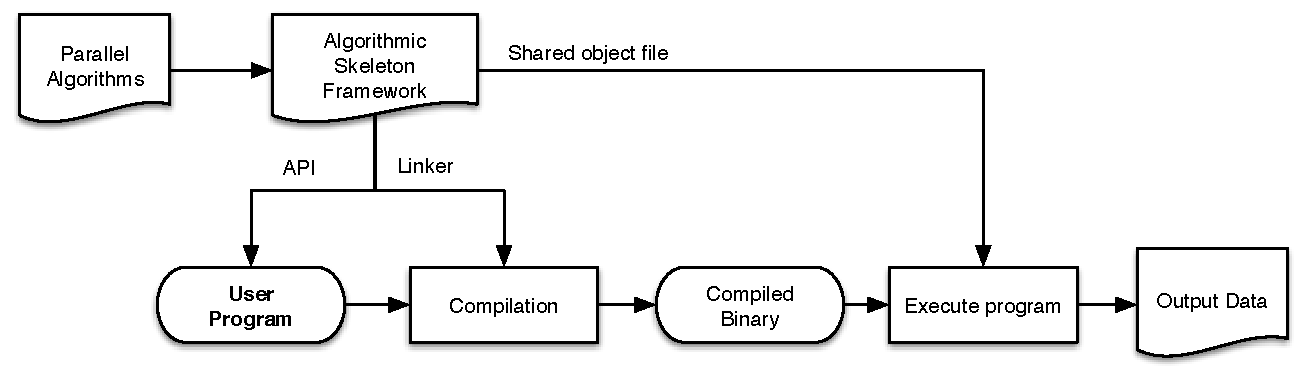
\includegraphics[width=0.99\textwidth]{img/askf}
\caption[Overview of an Algorithmic Skeleton Framework]{%
  Typical usage of a library based Algorithmic Skeleton
  Framework. Other approaches to Algorithmic Skeletons involve
  embedding the API into the core language itself, or using template
  and macro substitution to remove the need for linking with a
  library.%
}
\label{fig:askf}
\end{figure}

Algorithmic Skeleton Frameworks (ASkFs) provide concrete parallel
implementations of a set of parallel patterns, which are parameterised
by the user to generate specific problem solving programs. The
interfaces exposed by frameworks must be sufficiently generic to allow
users to express a range of problems.

Implementations of Algorithmic Skeletons abound, targeting a range of
different use cases and host languages. Notable examples include:
eSkel~\cite{Benoit2005a}, Skandium~\cite{Leyton2010}, and
FastFlow~\cite{Aldinucci2011}. The most prevalent form of ASkF is as a
standalone library built within a host library, which exposes a set of
APIs, shown in Figure~\ref{fig:askf}. See~\cite{Gonzalez2010} for a
more exhaustive review of ASkFs in the research literature.

In industry, Google's MapReduce~\cite{Dean2008} and Intel's Thread
Building Blocks~\cite{IntelTBB} have utilised a similar approach to
abstracting the coordination of parallel resources as in Algorithmic
Skeletons, to great commercial success, although they do not advertise
themselves as such.


\section{GPGPU Programming}\label{sec:gpgpu}

General purpose programming with graphics hardware is a nascent field,
but has shown to enable massive data parallel throughput by
re-purposing the hardware traditionally dedicated to the rendering of
3D graphics for generic computation. This was enabled by hardware
support for programmable shaders replacing the fixed function graphics
pipeline, and support for floating point operations in
2001. \citeauthor{Owens2006} provide a review of the first five years
of general purpose computation on graphics hardware
in~\cite{Owens2006}.

In the ensuing progress towards increasingly programmable graphics
hardware, two dominant programming models have emerged: CUDA and
OpenCL, which both abstract the graphics primitives of GPU hardware
and provide a platform for GPGPU programming. CUDA is a language
developed by NVIDIA for programming their GPUs using a proprietary SDK
and API~\cite{Nvidia2007}, while OpenCL is a vendor-independent open
standard based on a subset of the ISO C99 programming language, with
implementations for devices from most major GPU
manufactures~\cite{Stone2010}. Quantitative evaluations of the
performance of CUDA and OpenCL programs suggest that performance is
comparable between the two systems, although the wider range of target
architectures for OpenCL means that appropriate optimisations must be
made by hand or by the compiler~\cite{Komatsu2010,Karimi2010}.


\subsection{The OpenCL Programming Model}

\begin{figure}
\centering
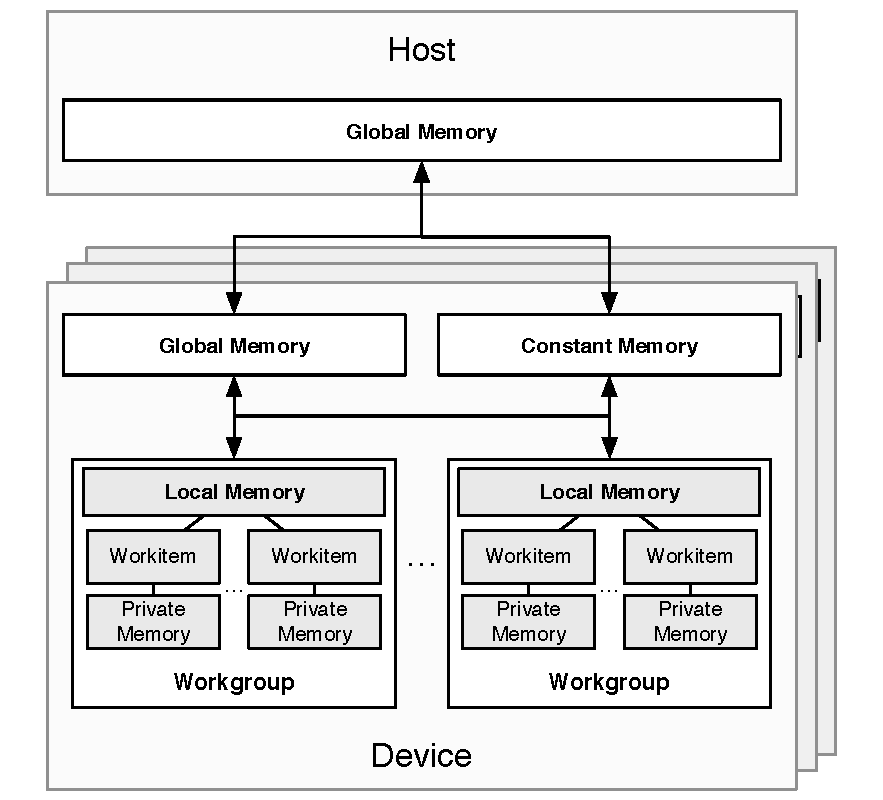
\includegraphics[width=0.5
\textwidth]{img/opencl-memory}
\caption[OpenCL memory model]{%
  The OpenCL memory model. The host communicates with each device
  through transfers between global memory spaces. The capacity of each
  type of memory is dependent on the device hardware. In general,
  private memory is the fastest and smallest, and global memory is the
  largest and slowest.%
}
\label{fig:opencl-memory}
\end{figure}

OpenCL is a parallel programming framework which targets CPUs, GPUs,
and other parallel processors such as Field-Programmable Gate
Arrays. It provides a set of APIs and a language (based on an extended
subset of C) for controlling heterogeneous \emph{compute devices} from
a central host. Programs written for these devices are called
\emph{kernels}, and are compiled by platform-specific tool chains. At
runtime, an OpenCL \emph{platform} is selected and a \emph{context}
object is created which exposes access to each supported compute
device through \emph{command queues}.  When a kernel is executed, each
unit of computation is referred to as a \emph{workitem}, and these
work items are grouped into \emph{workgroups}. The sum of all
workgroup dimensions defines the \emph{global size}. For GPUs,
workgroups execute on the Single Instruction Multiple Data (SIMD)
processing units in lockstep. This can cause a severe performance
penalty for flow control across workgroups, as ``thread masks'' must
be used to stall the execution of workitems across diverging branches.


\subsubsection{Memory Model}

Unlike the flat memory model of CPUs, OpenCL uses a hierarchical
memory model. The host and each OpenCL device has a single global
memory address space. Each workgroup has a local memory space, and
each workitem has a region of private memory.

Workgroups cannot access the memory of neighbouring workgroups, nor
can workitems access the private memory of other workitems. OpenCL
provides synchronisation barriers to allow for communication between
workitems within a single workgroup via the local memory, but not
global barriers. Memory transfers between the host and devices occurs
between global memory regions. In the case of programming
heterogeneous devices, these transfers must occur over the connection
bus between the CPU and device (e.g.\ PCIe for discrete GPUs), which
typically creates a performance bottleneck by introducing a
performance overhead to transfer data to the device for processing,
than back to the device afterwards. Direct transfers of data between
devices is not supported, requiring an intermediate transfer to the
host memory.


\subsubsection{Performance Optimisations}

The wide range of supported execution devices and differing
standard-compliant implementations makes portable performance tuning
of OpenCL programs a difficult task~\cite{Rul2010}, and the
interactions between optimisations and the hardware are complex and
sometimes counter-intuitive~\cite{Ryoo2008}.

The overhead introduced by memory transfers between host and compute
devices further complicates comparisons of OpenCL performance on
different devices. The conclusion of~\cite{Gregg2011} is that this
overhead can account for a $2\times$ to $50\times$ difference of GPU
program runtime. In~\cite{Lee2010}, \citeauthor{Lee2010} present a
performance analysis of optimised throughput computing applications
for GPUs and CPUs. Of the 14 applications tested, they found GPU
performance to be $0.7\times$ to $14.9\times$ that of multi-threaded
CPU code, with an average of only 2.5$\times$. This is much lower than
the $100\times$ to $1000\times$ values reported by other studies, a
fact that they attribute to uneven comparison of optimised GPU code to
unoptimised CPU code, or vice versa. \citeauthor{Lee2010} found that
multithreading, cache blocking, reordering of memory accesses and use
of SIMD instructions to contribute most to CPU performance. For GPUs,
the most effective optimisations are reducing synchronization costs,
and exploiting local shared memory. In all cases, the programs were
optimised and hand-tuned by programmers with expert knowledge of the
target architectures. It is unclear whether their performance results
still hold for subsequent generations of devices.

Despite the concerns of over-represented speedups, the potential for
high performance coupled with the complexity and low levels of
abstraction provided by OpenCL make it an ideal target for skeletal
abstractions. SkelCL and SkePU are two such examples which add a layer
of abstraction above OpenCL and CUDA respectively in order to simplify
GPGPU programming~\cite{Enmyren2010}.

\section{High-Level GPU Programming with
  SkelCL}\label{sec:skelcl-intro}

Introduced in~\cite{Steuwer2011}, SkelCL is an object oriented C++
library that provides OpenCL implementations of data parallel
algorithmic skeletons for heterogeneous parallelism using CPUs or
multi-GPUs. SkelCL addresses the parallel programmability challenge by
allowing users to easily harness the power of GPUs and CPUs for data
parallel computing.

The goal of SkelCL is to enable the transition towards higher-level
programming of GPUS, without requiring users to be intimately
knowledgeable of the concepts unique to OpenCL programming, such as
the memory or execution model~\cite{Steuwer2012}. SkelCL has been
shown to reduce programmer effort for developing real applications
through the use of robust pattern implementations and automated memory
management, with performance is within 5\% of equivalent
implementations hand written in OpenCL~\cite{Steuwer2013}.

OpenCL skeletons are parameterised with muscle functions by the user,
which are compiled into kernels for execution on device
hardware. SkelCL supports operations on one or two dimensional arrays
of data, with the Vector and Matrix container types transparently
handling communication between the host and device memory, and
supporting partitioning for multi-GPU
execution~\cite{Steuwer2013a}. SkelCL is freely
available\footnote{\url{http://skelcl.uni-muenster.de}} and
distributed under dual GPL and academic licenses.


\subsection{Pattern definitions}

SkelCL provides six skeletons for data parallel operations: $\map$,
$\zip$, $\reduce$, $\scan$, $\allpairs$, and $\stencil$. The focus of
this thesis is on tuning the $\stencil$ skeleton, but for the sake of
completeness I provide here a brief overview of the behaviour of all
six.


\subsubsection{Map}

The $\map$ operation is a basic building block of data parallel
algorithms. Given a customising function $f$ and a vector $x$ of $n$
elements, the $\map$ operation applies the function $f$ to each
element $x_1, x_2, \ldots, x_n$, return a vector of the same length:
%
\begin{equation}
\map\left(f, [x_1,x_2,\ldots,x_n]\right) \to [f(x_1),f(x_2),\ldots,f(x_n)]
\end{equation}
%
The process is the same for an $n \times m$ matrix:
%
\begin{equation}
\map\left(f,
\begin{bmatrix}
  x_{11} & \cdots & x_{1m} \\
  \vdots & \ddots & \vdots \\
  x_{n1} & \cdots & x_{nm}
\end{bmatrix}\right)
\to
\begin{bmatrix}
  f(x_{11}) & \cdots & f(x_{1m}) \\
  \vdots & \ddots & \vdots \\
  f(x_{n1}) & \cdots & f(x_{nm})
\end{bmatrix}
\end{equation}
%
Execution of the customising function can be parallelised as each are
independent of each. There is no guarantees on execution on ordering.


\subsubsection{Zip}

The $\zip$ operation combines elements of containers pairwise. Given a
binary operator $\oplus$ and two vectors $x$ and $y$ of $n$ elements
each:
%
\begin{equation}
\zip\left( \oplus, [x_1,x_2,\ldots,x_n], [y_1,y_2,\ldots,y_n] \right)
\to
\left[ x_1 \oplus y_1, x_2 \oplus y_2, \ldots, x_n \oplus y_n \right]
\end{equation}
%
For two matrices of $n \times m$ elements each:
%
\begin{equation}
\begin{split}
\zip \left( \oplus,
\begin{bmatrix}
  x_{11} & \cdots & x_{1m} \\
  \vdots & \ddots & \vdots \\
  x_{n1} & \cdots & x_{nm}
\end{bmatrix},
\begin{bmatrix}
  y_{11} & \cdots & y_{1m} \\
  \vdots & \ddots & \vdots \\
  y_{n1} & \cdots & y_{nm}
\end{bmatrix} \right) \\
\to
\begin{bmatrix}
  x_{11} \oplus y_{11} & \cdots & x_{1m} \oplus y_{1m} \\
  \vdots & \ddots & \vdots \\
  x_{n1} \oplus y_{n1} & \cdots & x_{nm} \oplus y_{nm}
\end{bmatrix}
\end{split}
\end{equation}
%
It is parallelised in the same manner as $\map$.


\subsubsection{Reduce}

The $\reduce$ operator combines all elements of an input vector and
returns a scalar. Given a binary operator $\oplus$, its identity
$\bm{i}$ and a vector $x$ of $n$ elements:
%
\begin{equation}
  \reduce \left( \oplus, \bm{i}, [x_1,x_2,\ldots,x_n] \right)
  \to
  x_1 \oplus x_2 \oplus \ldots \oplus x_n
\end{equation}
%
For a $n \times m$ matrix:
%
\begin{equation}
\reduce \left( \oplus, i,
\begin{bmatrix}
  x_{11} & \cdots & x_{1m} \\
  \vdots & \ddots & \vdots \\
  x_{n1} & \cdots & x_{nm}
\end{bmatrix} \right)
\to
x_{11} \oplus x_{12} \oplus \ldots \oplus x_{nm}
\end{equation}
%
Reduction operates recursively combines elements, storing intermediate
results in fast local memory. No guarantee is made on execution
ordering, so the binary operator must be associative.


\subsubsection{Scan}

The $\scan$ operator applies a binary function $\oplus$ to each member
of an input array $x$ of $n$ elements, such that element $x_i$ at the
$i$th position is calculated by applying the binary function to all
elements $x_1,x_2, \ldots x_{i-1}$. For the first element $x_i$, the
value is the identify $\bm{i}$ of the $\oplus$ operator:
%
\begin{equation}
  \scan \left( \oplus, i, [x_1,x_2,\ldots,x_n] \right)
  \to
  \left[ \bm{i}, x_1, x_1 \oplus x_2, \ldots, x_1 \oplus x_2 \oplus \ldots \oplus x_n \right]
\end{equation}
%
The SkelCL scan implementation is heavily optimised to make use of
local memory, based on the design from~\cite{Harris2007a}.


\subsubsection{AllPairs}

The AllPairs skeleton is a specialised pattern for Matrix Matrix
operations, introduced in~\cite{Steuwer2014}. Given an two matrices of
size $n \times d$ and $n \times m$, a binary operator $\oplus$:
%
\begin{equation}
\allpairs \left( \oplus,
\begin{bmatrix}
  x_{11} & \cdots & x_{1d} \\
  \vdots & \ddots & \vdots \\
  x_{n1} & \cdots & x_{nd}
\end{bmatrix},
\begin{bmatrix}
  y_{11} & \cdots & y_{1m} \\
  \vdots & \ddots & \vdots \\
  y_{n1} & \cdots & y_{nm}
\end{bmatrix} \right)
\to
\begin{bmatrix}
  z_{11} & \cdots & z_{1m} \\
  \vdots & \ddots & \vdots \\
  z_{n1} & \cdots & z_{nm}
\end{bmatrix}
\end{equation}
%
where:
%
\begin{equation}
z_{ij} =
\left[ x_{i1}, x_{i2}, \ldots, x_{id} \right] \oplus
\left[ y_{j1}, y_{j2}, \ldots, y_{jd} \right]
\end{equation}
%
An additional implementation is provided for when the $\oplus$
operator is known to match that of a zip pattern:
%
\begin{equation}
z_{ij} =
\left[
  x_{i1}, \oplus y_{j1}, x_{i2} \oplus y_{j2}, \ldots, x_{id} \oplus y_{jd}
\right]
\end{equation}
%
This pattern has applications from bioinformatics to matrix
multiplication, and uses fast local memory to reduce data access times
for repeated reads.


\subsubsection{Stencil}

\begin{figure}
\centering
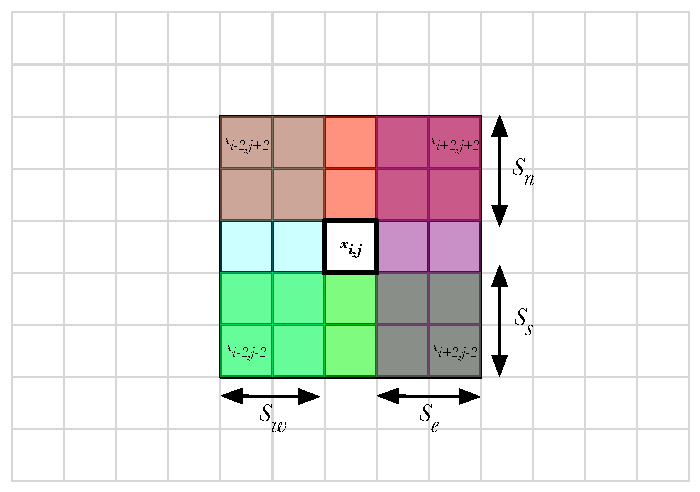
\includegraphics[width=.6\textwidth]{img/stencil-shape}
\caption[Stencil border region]{%
  The border region of a stencil is defined using a stencil shape $S$,
  consisting of the four independent components describing the number
  of cells north $S_n$, east $S_e$, west $S_w$, and south $S_s$.%
}
\label{fig:stencil-shape}
\end{figure}

Stencils are patterns of computation which operate on uniform grids of
data, where the value of each cell is updated based on its current
value and the value of one or more neighbouring elements, called the
\emph{border region}. Introduced in~\cite{Breuer2014}, SkelCL provides
a 2D stencil skeleton which allows users to provide a function which
updates a cell's value; while SkelCL orchestrates the parallel
execution of this function across all cells.

The border region is described by a \emph{stencil shape}, which
defines an $i \times j$ rectangular region about each cell which is
used to update the cell value. Stencil shapes may be asymmetrical, and
are defined in terms of the number of cells in the border region to
the north, east, south, and west of each cell, shown in
Figure~\ref{fig:stencil-shape}.

Given a customising function $f$, a stencil shape $S$, and an
$n \times m$ matrix:
%
\begin{equation}
\stencil \left( f, S,
\begin{bmatrix}
  x_{11} & \cdots & x_{1m} \\
  \vdots & \ddots & \vdots \\
  x_{n1} & \cdots & x_{nm}
\end{bmatrix} \right)
\to
\begin{bmatrix}
  z_{11} & \cdots & z_{1m} \\
  \vdots & \ddots & \vdots \\
  z_{n1} & \cdots & z_{nm}
\end{bmatrix}
\end{equation}
%
where:
%
\begin{equation}
z_{ij} = f \left(
\begin{bmatrix}
  z_{i-S_n,j-S_w} & \cdots & z_{i-S_n,j+S_e} \\
  \vdots & \ddots & \vdots \\
  z_{i+S_s,j-S_w} & \cdots & z_{i+S_s,j+S_e}
\end{bmatrix} \right)
\end{equation}
%
Note that a stencil operation in which the size of the stencil shape
$S$ is zero in every direction is functionally equivalent to a $\map$
operation. Where the a border region includes elements outside of the
matrix, values are substituted from either a predefined padding value,
or the value of the nearest cell within the matrix. The choice of
which is determined by the user.

A popular usage of Stencil codes is for solving problems iteratively,
whereby a stencil operation is repeated over a range of discrete time
steps $0 \le t \le t_{max}$, and $t \in \mathbb{Z}$. An iterative
stencil operation $g$ accepts a customising function $f$, a Stencil
shape $S$, and a matrix $M$ with initial values $M_{init}$. The
iterative stencil can be defined recursively as:
%
\begin{equation}
g(f, S, M, t) =
\begin{cases}
  \stencil \left( f, S, g(f, S, M, t-1) \right),& \text{if } t \geq 1\\
  M_{init}, & \text{otherwise}
\end{cases}
\end{equation}
%
Examples of iterative stencils are cellular automata. Another
extension of the stencil operation accepts an ordered list of
customising functions which are applied sequentially for each
iteration. This has applications for multi-stage stencil operations
such as Canny Edge Detection, in which four distinct stencil
operations are performed as a sequence.


\subsection{Implementation Details}

Each skeleton is represented by a template class, declared in a header
file detailing the public API, e.g.\ \texttt{SkelCL/Stencil.h}. A
private header file contains the template class declaration, e.g.\
\texttt{SkelCL/detail/StencilDef.h}. Small OpenCL kernels are stored
as inline strings inside the definition headers. Non-trivial OpenCL
kernels are stored in separate source files, e.g.\
\texttt{SkelCL/detail/StencilKernel.cl}. Muscle functions are passed
as OpenCL strings to the skeleton template classes, and the LLVM API
is used to perform argument and function name substitution.

\subsubsection{Stencil Implementation}

For the stencil skeleton, each cell maps to a single work item; and
this collection of work items is then divided into \emph{workgroups}
for execution on the target hardware. In a stencil code, each
work-item reads the value of the corresponding grid elements, and the
surrounding elements defined by the border region. Since the border
regions of neighbouring elements overlap, the value of all elements
within a workgroup are stored in a \emph{tile}, which is a region of
local memory. As local memory access times are much smaller than that
of global memory, this greatly reduces the latency of the border
region reads performed by each workitem. Changing the workgroup size
thus affects the amount of local memory required for each workgroup,
which in turn affects the number of workgroups which may be
simultaneously active. So while the user defines the size, type, and
border region of the of the grid being operated upon, it is the
responsibility of the SkelCL stencil implementation to select an
appropriate workgroup size to use.

\begin{figure}
\centering
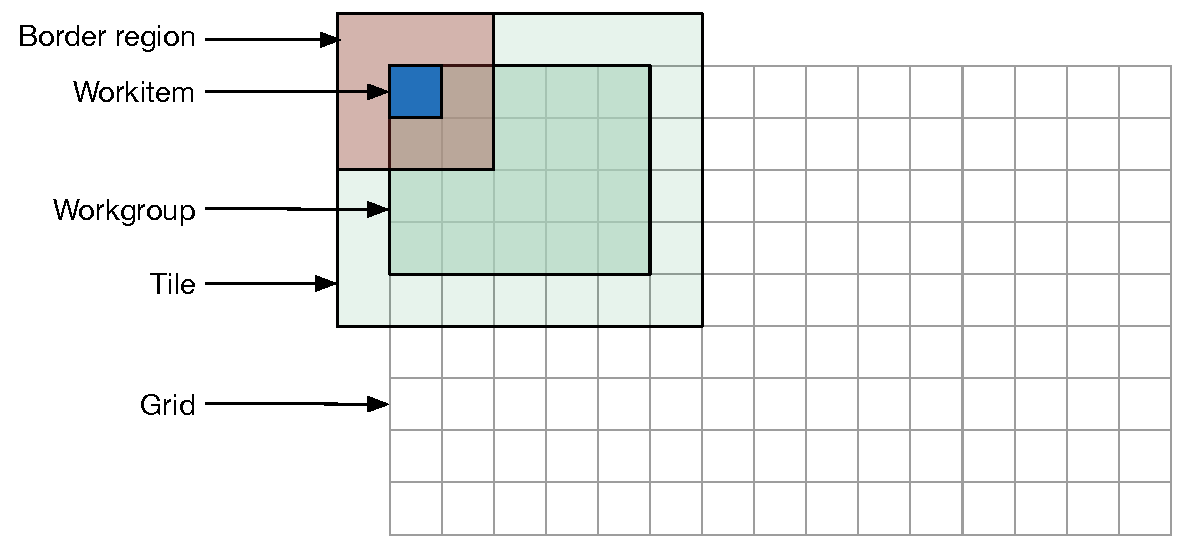
\includegraphics[width=.75\textwidth]{img/stencil-wg}
\caption[Workgroup decomposition in stencils]{%
  The components of a stencil: a grid of cells is decomposed into
  workgroups, consisting of multiple workitems. Each work item
  operates on a border region, and the size of the workgroup and outer
  border region defines a tile, which is a region of local memory
  allocated to each workgroup.%
}
\label{fig:stencil-wg}
\end{figure}


\section{Machine Learning}


Multiple machine learning methods are used in this thesis to perform
classification and regression tasks. Classification is the task of
predicting the correct category --- or class --- for a new instance,
based on ``labelled'' training data, i.e.\ instances whose categories
are known. The properties describing instances are called
\emph{features}. The purpose of regression is to predict the
relationship between a dependent variable, and the value of one or
more independent variables. Unlike with classification, the predicted
dependent variable can be continuous, rather than categorical. This
section briefly describes the properties of classifiers and regressors
used in this thesis.


\subsubsection{ZeroR}

A ``ZeroR'' classifier represents the simplest approach to
classification, in that it ignores all features, and simply predicts
the mode of the training data labels. This is useful for providing a
baseline to evaluate the performance of more complex classifiers
against, since a ZeroR classifier has no power of prediction.


\subsubsection{Naive Bayes}

Naive Bayes classifiers are probabilistic classifiers which assume
strong independence between features. That is, the value of one
feature is considered independently of another, and is what lends the
\emph{Naive} portion of the name. The goal of Naive Bayes is to
predict the probability of a class $y$, given a set of $d$ independent
variables $x = x_1, x_2, \ldots x_d$. Naive Bayes applies Bayes
theorem, which states that given a \emph{prior} (i.e.\ unconditional)
probability for each class $P(y)$, a class-\emph{conditional} model
$P(x|y)$, and a normaliser $P(x) = \sum_{y'}P(x|y')P(y')$, the
probability of a class $y$ given variables $x$ is equal to the
probability of $x$ given $y$, multiplied by the probability of $y$:
%
\begin{equation}
  P(y|x) = \frac{P(x|y)P(y)}{\sum_{y'}P(x|y')P(y')}
\end{equation}
%
The class which has the highest probability from the set of possible
classes $Y$ is the prediction. Note that the normaliser $P(x)$ does
not affect the class which is most likely. The class conditional model
uses ``counts'' for each observation based on training data:
%
\begin{equation}
  P(x|y) = \prod_{i=1}^{d} P(x_i|y)
\end{equation}
%
The simplicity of Naive Bayes makes it attractive for various purposes
such as text classification (using word frequency as features), but
the assumption of independence means that it is not universally
successful.


\subsubsection{Decision Trees}

Decision trees are an intuitive form of classification in which a tree
structure of decision nodes are used to predict the class for a given
set of features.

Given a set of examples $D$, and $p_{(+)}$ and $p_{(-)}$ are the
number of positive and negative examples in $D$:

\begin{equation}
  H(D) = - p_{(+)}\log_2p_{(+)} - p_{(-)}\log_2p_{(-)}
\end{equation}

\begin{equation}
  \gain(D, A) = H(D) - \sum_{V \in \text{Values}(A)}\frac{|D_V|}{|D|}H(D_V)
\end{equation}

Decision trees are very popular and low overhead form of
classification, as they can be implemented using a nested set of
\texttt{if}/\texttt{else} statements. However, they often have an
issue of overfitting to the training data, if preventative action is
not taken.


\subsubsection{Random Forest}

Random Forests are an ensemble technique which attempt to overcome the
tendency of decision trees to overfit training by training multiple
decision trees and using the mode of each tree to select
predictions~\cite{Breiman1999}. If trained using regression trees,
Random Forests are capable of regression, in which the predicted
values are the mean of all trees.

\subsubsection{Logistic Regression}


\subsubsection{SMO}



\section{Statistics}

This section describes a number of the statistical tools used
throughout this thesis.

% \subsubsection{Statistical Testing}

% Student's \emph{t}-test


\subsubsection{Interquartile Range}

For a given set of ordered data values, the quartiles are the three
points that divide the data set into four groups of equal size. The
first quartile is the point which $Q_1$ divides the data equally
between the lowest value and the median, $Q_2$. The third quartile
$Q_3$ is the point which divides the data between the median and the
highest value. The interquartile range (IQR) measures the dispersion
of a data set, and is the difference between the third and first
quartiles, $Q_3 - Q_1$.


\subsubsection{Confidence Intervals}

Confidence intervals estimate the interval for the true range of a
population parameter. Given a set of samples of a population with
estimates of a parameter value for each, the confidence interval
$(c_1,c_2)$ estimates the frequency that the true parameter value will
fall between the per-sample confidence interval. Given a sample $x$
with sample size $n$, the confidence interval for a confidence
$\alpha$ is found using:
%
\begin{align}
  \bar{x} &= \frac{1}{n}\sum_{i=1}^{n} x_i\\
  \sigma &= \sqrt{\frac{\sum_{i=1}^{n}(x_i - \bar{x})^2}{n - 1}}\\
  c_1 &= \bar{x} - z_{1-\alpha/2}\frac{\sigma}{\sqrt{n}}\\
  c_2 &= \bar{x} + z_{1-\alpha/2}\frac{\sigma}{\sqrt{n}}
\end{align}
%
Where the value $z_{1-\alpha/2}$ assumes a Gaussian distribution of
the underlying data, and the values for popular $\alpha$ values are
typically found using pre-computed ``Z-tables''. To calculate
confidence intervals for the ratio of two means, $\bar{x}_1$ and
$\bar{x}_2$ with sample sizes $n_1$ and $n_2$, and respective standard
deviations $\sigma_1$ and $\sigma_2$:
%
\begin{align}
  \sigma_x &= \sqrt{\frac{\sigma_1^2}{n_1} + \frac{\sigma_2^2}{n_2}}\\
  c_1 &= \bar{x}_1 - \bar{x}_2 - z_{1-\alpha/2}\sigma_x\\
  c_2 &= \bar{x}_1 - \bar{x}_2 + z_{1-\alpha/2}\sigma_x
\end{align}
%
The above calculations assumes that the sample variance ($\sigma^2$)
is an accurate estimation of the true population variance. This relies
on the assumption of an underlying Gaussian distribution, which,
according to the central limit theorem, is true of large sample sizes
(typically $n \ge 30$).  In cases of smaller sample sizes, the sample
and population variances can differ significantly, so one must instead
use a Student's $t$-distribution, $t_{1-\alpha/2}$, in place of
$z_{1-\alpha/2}$.


\subsubsection{Histogram}

Histograms are a widely used statistical visualisation which shows the
distribution of numerical data. The data is first divided into a set
of discrete, equally sized sub-intervals, or \emph{bins}. The number
of data points in each bin is used to show visualise the density
distribution. The shortcoming of histograms is that their appearance
is heavily influenced by three user-selected parameters: the number of
bins, the width of bins (binwidth), and the endpoints chosen. As such,
they may provide a misleading representation of the data if
inappropriate values for any of these parameters are chosen. Kernel
Density estimation is a technique for showing the distribution of data
which circumvents some of these issues.


\subsubsection{Kernel Density Estimation}

A Kernel Density Estimate (KDE) is an approximation of the probability
density function of a random variable. Given a random variable $x$,
and bandwidth $h$ and a kernel $K$, the Kernel Density Estimate
$\hat{f}_h(x)$ can be found using:
%
\begin{equation}
  \hat{f}_h(x) = \frac{1}{nh} \sum^{n}_{i=1} K\left( \frac{x - x_i}{h} \right)
\end{equation}
%
Using a smooth kernel such as a Gaussian distribution for the kernel
produces a smooth density estimated, unlike histograms. However, like
histograms, the appearance of a Kernel Density Estimate plot is
dependent on the value of the bandwidth parameter $h$ (equivalent to
binwidth in histograms), so care must be taken to select a value to
minimise over or under smoothing. Grouped data can be shown by
plotting multiple KDEs on the same axes, although if the number of
groups is large, a box plot or violin plot may be more appropriate.


\subsubsection{Box plot}

Box plots are used to show the distribution of quartile ranges for
grouped data. The contain the following features:
%
\begin{itemize}
\item Horizontal lines at the lower quartile, median and upper
  quartile.
\item Vertical lines above and below the upper and lower quartiles to
  the most extreme data point within 1.5 IQR of the upper/lower
  quartile, with horizontal whiskers at the end of the vertical lines.
\item Dots beyond the ends of the vertical lines to show outliers.
\end{itemize}
%
A variation of box plots used in this thesis is the violin plot, which
extends the box plot with a fitted Kernel Density Estimate plot to
show the probability \emph{density} of data at different values. To
construct a violin plot, KDEs for each group are rotated and mirrored
to generate a smoothed visualisation of the distribution.


\section{Summary}

This chapter gave a brief introduction to general-purpose computing
using graphics hardware, the OpenCL framework, and SkelCL. It was
followed by a description of the machine learning techniques used
throughout this thesis, and the statistical tools used for the
evaluation. In the next chapter, I review the state of the art in the
field of autotuning, and provide context for the contributions of this
thesis.
